\paragraph{}
After the geometry information is exported from the IGES file, it can be feed into the quad-tree algorithm to generate mesh of the problem domain.
As an algorithm based on computational geometry, it require great amount of numerical operation and hence the result may be sensitive to the tolerance.
An absolute tolerance may not be able to handle problem with very large or small geometric size.
As a consequence, the first step is to normalize the geometry into a uniform space ($10\times10$ is used in this chapter).

\subsection{Background mesh}
\paragraph{}
Background mesh, like its name, describe a mesh in the background. %fig
Its density is decided by the geometry.
This section will introduce the procedure to generate the background mesh.
\paragraph{}
First of all, we start with one square which is the root of the tree.
The size of it will be slightly larger than the normalized input geometry and it is selected as $16 \times 16$ in this chapter.
After that, the root square will be divided into millions (defined by resolution, defined as $2^{res} \times 2^{res}$) smaller ones like pixels in the image.
Then, $2^{s_{max}} \times 2^{s_{max}}$ ``pixels'' will be group into the first layer of the tree, or initial background mesh as shown in fig.~\ref{qdt_fig:qdt_initial_mesh}.
It is used to control the maximum allowable mesh size globally or separately for different material regions.

\begin{figure}[!ht]
    \centering
    \scalebox{0.8}{
        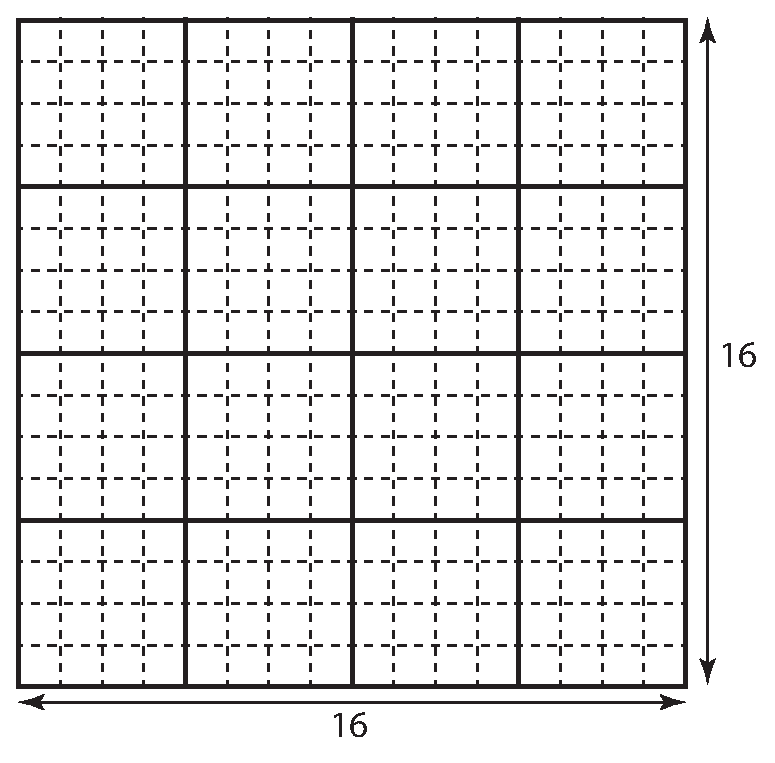
\includegraphics{quadtree/images/qdt_initial_mesh.eps}
    }
    \caption{An example of the background initial mesh: $16 \times 16$ square are divided into $2^4 \times 2^4$ pixels (dashed lines, $res=4$) and $2^2 \times 2^2$ pixels form the initial mesh (solid lines, $s_{max}=2$)}
    \label{qdt_fig:qdt_initial_mesh}
\end{figure}

\paragraph{}
There are two ways to decided whether each individual square need to be refined or not, seed points method and curve size field and both of them will be used depends on the requirement of the controlling over the mesh.

\paragraph{}


\subsection{Hardpoint treatment}

\subsection{Bucket sort algorithm}

\subsection{Cutting with boundary}

\subsection{Color the region}
